\section{Resultados}


\subsection{Tests} %como corren los tests y si hay nuevos

  El codigo implementado pasa todos los tests, se realizo un nuevo test el cual utiliza
  archivos generados aleatoriamente y compara los resultados de las dos funciones
  de maximos implementadas.

  esto tambien cumple la funcion de medir sus tiempos de ejecucion varias veces,
  este test fue modificado para trabajar con muchos archivos o con pocos y comparar
  el desempeño de ambos algoritmos, mas adelante
  se hablara de estas mediciones.

\subsubsection{Tiempos de ejecucion} %diferencias entre los 2 maximos

\begin{center}
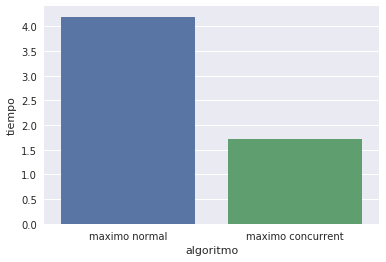
\includegraphics[width=0.8\textwidth]{imagenes/maxvsmax.png}
\end{center}

en este grafico se puede ver la comparacion entre las dos implementaciones de maximo funcionando
para 5 archivos con 5 threads, se puede ver claramente que la implementacion concurrente
es mas del doble de rapida.

\begin{center}
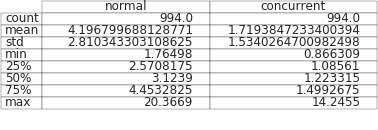
\includegraphics[width=0.8\textwidth]{imagenes/descplot.png}
\end{center}

en esta tabla se pueden ver los valores mas estadisticos de la comparacion, se
corrieron aproximadamente mil veces los algoritmos para este caso.


\begin{center}
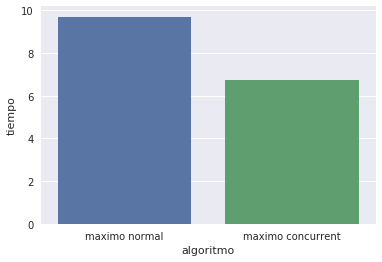
\includegraphics[width=0.8\textwidth]{imagenes/maxvsmax1thread.png}
\end{center}

Aqui se puede ver la comparacion de ambos para 11 archivos con 1 solo thread. la diferencia es menor
pero igualmente es claro que la implementacion concurrente es mejor

\begin{center}
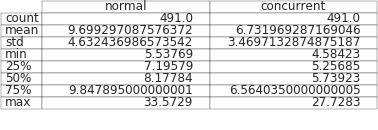
\includegraphics[width=0.8\textwidth]{imagenes/descplot2.png}
\end{center}

en esta tabla se pueden ver los valores mas estadisticos de la comparacion, en este caso
los algorimos se corrieron aproximadamente quinientas veces.
